\documentclass[addpoints]{exam}

% \pagestyle{empty}                       %no page numbers
% \thispagestyle{empty}                   %removes first page number
% \setlength{\parindent}{0in}               %no paragraph indents

\usepackage{fullpage}
\usepackage[tmargin = 0.5in, bmargin = 1in, hmargin = 1in]{geometry}     %1-inch margins
\geometry{letterpaper}                  
\usepackage{graphicx}
\usepackage{amssymb}

% Default packages
\usepackage{latexsym}
\usepackage{amsfonts}
\usepackage{amsmath}
\usepackage{amsthm}
\usepackage{hyperref}
\usepackage{multicol}
\usepackage{multirow}
\usepackage{enumerate}
\usepackage{enumitem}


%% Definitions
\def\va{\mathbf{a}}
\def\vb{\mathbf{b}}
\def\vc{\mathbf{c}}
\def\vx{\mathbf{x}}
\def\vzero{\mathbf{0}}



\def\vi{\mathbf{i}}
\def\vj{\mathbf{j}}
\def\vk{\mathbf{k}}
\def\vr{\mathbf{r}}
\def\vu{\mathbf{u}}
\def\vv{\mathbf{v}}
\def\pageturn{\vfill
\begin{flushright}
	\begin{small}
		Continued $\rightarrow$
	\end{small}
\end{flushright}
\newpage}

\pagestyle{headandfoot}
\runningheadrule
\firstpageheader{\textbf{MTH 201-03 (Talbert)}}{\textbf{In-Class Assessment 3 --- \numpoints \ points}}{\textbf{November 22, 2013}}
\runningheader{MTH 201}
{MTH 201-03 Assessment 3, Page \thepage\ of \numpages}
{Nov 22, 2013}
\firstpagefooter{}{}{}
\runningfooter{}{}{}

\begin{document}

		
\vspace*{0pt}

\noindent
Name: \underline{\hspace{2in}} \\


\noindent
\textbf{Instructions}:  You may use a $3 \times 5$ notecard with notes on it as well as a calculator. Except on multiple choice questions, you need to show all work in a clear and complete way to receive credit. The Assessment will end promptly at 2:50pm unless you have made alternate arrangements. 

\begin{questions}

\uplevel{\emph{Items 1---10 are multiple choice questions that address a variety of learning objectives. Please circle the ONE response you believe is most correct. You do not need to justify your answer.}}

\question[2] Which of the following statements is always true, for any continuous function $f$ whose domain is the entire real number line (i.e. not confined to a closed interval)? 
	\begin{parts}
		\part If $f$ has a local extreme value at $x=c$, then $f$ has a critical number at $x=c$. 
		\part If $f$ has a critical number at $x=c$, then $f$ has a local extreme value at $x=c$. 
		\part If $f$ is such that $f'(c) = 0$, then $f''(c) = 0$ too. 
		\part All of the above
		\part Just (a) and (c) 
	\end{parts}
	
\question[2] Which of the following statements is always true, for any continuous function $f$ whose domain is the entire real number line? 
	\begin{parts}
		\part If $f$ has a local extreme value at $x=c$, then $f$ has a global extreme value at $x=c$. 
		\part If $f$ has a global extreme value at $x=c$, then $f$ has a local extreme value at $x=c$. 
		\part If $f$ has a local extreme value at $x=c$, then $f$ has an inflection point at $x=c$. 
		\part All of the above
		\part Just (a) and (c) 
	\end{parts}

\question[2] Suppose $f$ is a function whose derivative is $f'(x) = \dfrac{x^2 - 1}{x^2}$. Then
	\begin{parts}
		\part $f$ has no critical values
		\part $f$ has one critical value
		\part $f$ has two critical values
		\part $f$ has three critical values
		\part $f$ has more than three critical values
	\end{parts}

\question[2] Suppose $k(x)$ is a function such that $k'(4) = 0$ and $k(4) = 3$. Then
	\begin{parts}
		\part The graph of $k$ touches the $x$-axis at $x=4$
		\part $k$ has a local minimum at $x = 4$
		\part $k$ has a local maximum at $x = 4$
		\part $k$ has neither a local minimum nor a local maximum at $x = 4$
		\part There is not enough information present to determine the behavior of $k$ at $x = 4$
	\end{parts}
	
\question[2] Suppose $g$ is a function such that $g'(3) = 0$ and $g''(3) > 0$. Then 
	\begin{parts}
		\part $g$ has a local minimum at $x = 3$
		\part $g$ has a local maximum at $x = 3$
		\part $g$ has an inflection point at $x = 3$
		\part All of the above
		\part None of the above
	\end{parts}
	
\pageturn

\question[2] Which of the following is an antiderivative for the function $f(x) = x + \dfrac{1}{x}$? 
	\begin{parts}
		\part $F(x) = 1 - \frac{1}{x^2}$
		\part $F(x) = x^2 + \ln(x)$
		\part $F(x) = \frac{x^2}{2} + \ln(x) - 10$
		\part Both (b) and (c)
		\part None of the above
	\end{parts}

\question[2] A continuous function whose domain is a closed interval
	\begin{parts}
		\part Must have a critical number inside the interval
		\part Must have a local extreme value inside the interval
		\part Must have a global extreme value inside the interval or at the endpoints of the interval
		\part All of the above 
		\part Just (a) and (c) 
	\end{parts}
	
\question[2] The family of functions $f(x) = cx^2 + x + 1$, where $c$ is a parameter,
	\begin{parts}
		\part Is increasing for all $x$ when $c > 0$ and decreasing for all $x$ when $c < 0$ 
		\part Is decreasing for all $x$ when $c > 0$ and increasing for all $x$ when $c < 0$ 
		\part Is concave up for all $x$ when $c > 0$ and concave down for all $x$ when $c < 0$ 
		\part Is concave down for all $x$ when $c > 0$ and concave up for all $x$ when $c < 0$ 
		\part None of the above
	\end{parts}
	
\question[2] In the process of calculating the Riemann sum $M_{8}$ for the function $f(x)$ on the interval $[1,2]$, the value of $\Delta x$
	\begin{parts}
		\part Equals $1/4$
		\part Equals $1/2$
		\part Equals $2$
		\part Equals $16$
		\part Cannot be determined without more information about $f$
	\end{parts}
	
\question[2] Under which of the following conditions will the Riemann sum $L_8$ be an overestimate for the area between the graph of a function $f$ and the $x$-axis on the interval $[a,b]$? 
	\begin{parts}
		\part $f$ is increasing on $[a,b]$
		\part $f$ is decreasing on $[a,b]$
		\part $f$ is concave up on $[a,b]$
		\part $f$ is concave down on $[a,b]$
		\part None of the above
	\end{parts}

%%%%%
% Begin problem section 
%%%%%

\pageturn

\uplevel{\emph{The next several items are problems to solve. Be sure to give complete, clear, and correct solutions to each, not just answers unless clearly specified.}}


\question[20] For some function $f(x)$, whose formula you do not have, it is known that 
\[ f'(x) = -xe^{-x} (x-2) \qquad \text{and} \qquad f''(x) = e^{-x}(x^2 - 4x + 2) \]
Construct well-labeled first and second derivative sign charts for $f(x)$, clearly labeling all critical points, relative extremes, and points of inflection, as well as the relevant behavior of $f$ in each appropriate interval. Use your work to construct a well-labeled possible graph of $f(x)$ on the axes provided, using the additional given fact that $f(0) = −2$.

\medskip

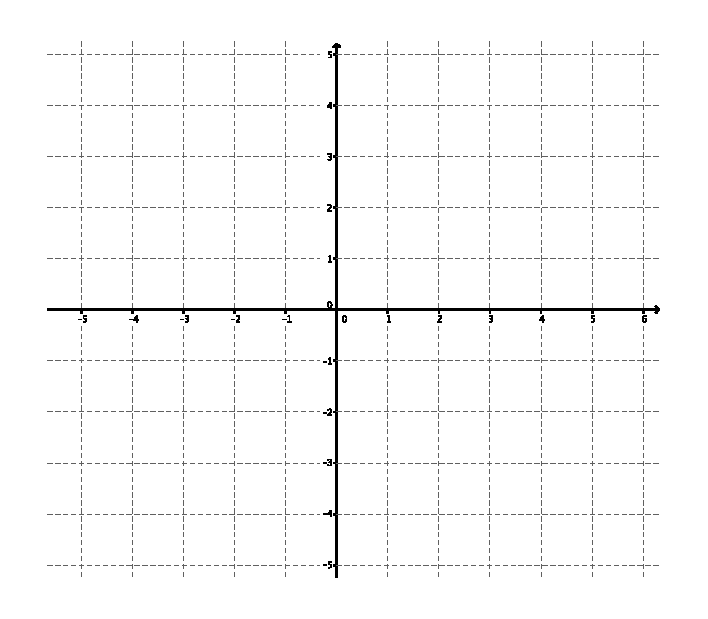
\includegraphics[width=0.6\textwidth]{a3-axes}


\pageturn

%\question[12] Family of functions

\question Suppose you want to make a fenced-in region like the one below: 
\begin{center}
	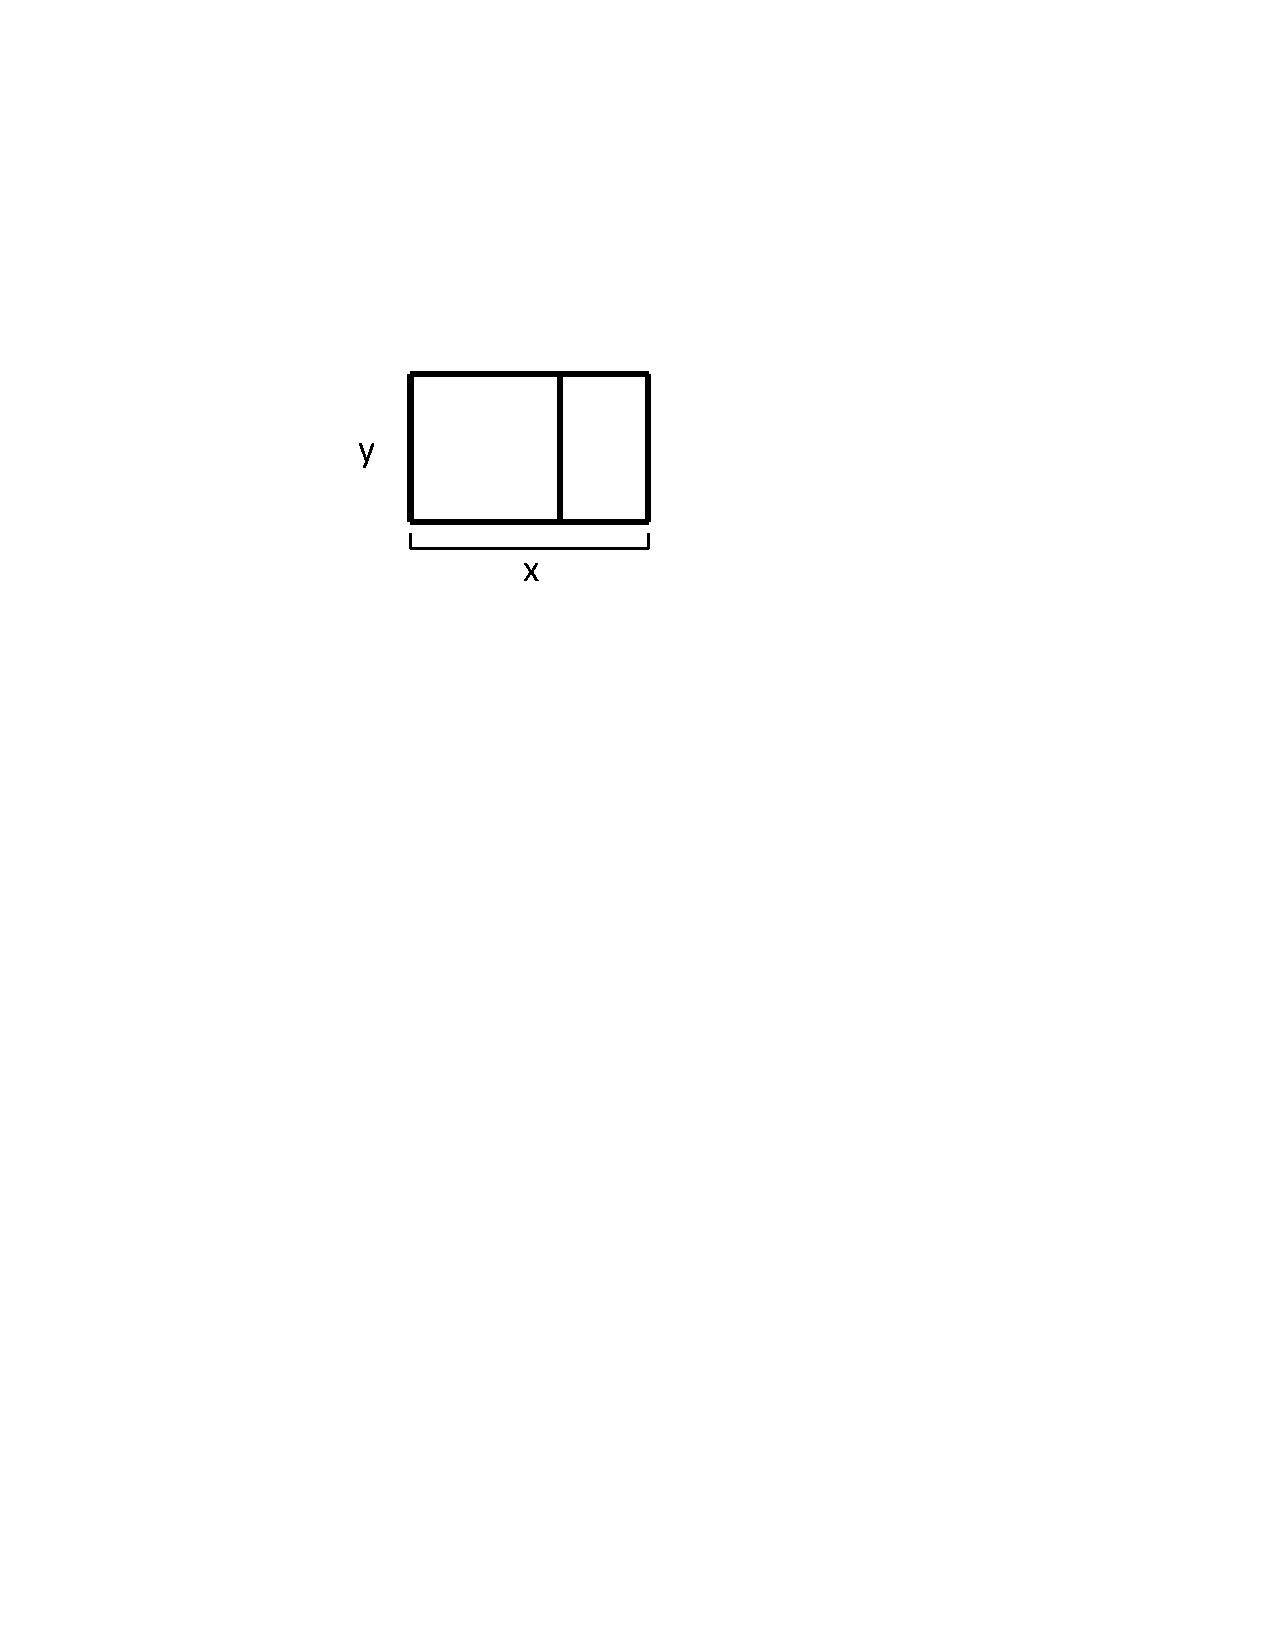
\includegraphics[width=2in]{a3-opt}
\end{center}
	\begin{parts}
		\part[4] What is the total length of the fence (including the fence on the inside) in terms of $x$ and $y$? 
		
		\vspace{1in}
		
		\part[4] What is the area of the fenced-in region in terms of $x$ and $y$? 
		
		\vspace{1in}
		
		
		\part[12] If you have to make the area of the fenced-in region 24 square feet, how should you build the fence in order to minimize the amount of fencing used? Make sure you justify that your answer actually produces a minimum. 
	\end{parts}
	
\pageturn

\question[20] Work EXACTLY ONE of the following problems. Clearly indicate which one you are doing and which one you are not doing; submitting significant work on both will result in a grade of ``0'' on this problem. Show all work and organize your solution clearly, as a narrative that explains the correctness to the reader using mathematics as support. You will lose credit for disorganized solutions. 
	\begin{itemize}
		\item If two resistors with resistances \(R_1\) and \(R_2\) are connected in parallel, as in the figure, then the total resistance \(R\), measured in Ohms \((\Omega)\), is given by:
		\[\displaystyle\frac{1}{R} =\frac{1}{R_1}+\frac{1}{R_2}\] \leavevmode\\\relax 
		If \(R_1\) and \(R_2\) are increasing at rates of \(.3\,\Omega/s\) and \(.2\, \Omega/s\), respectively, how fast is \(R\) increasing when \(R_1=80\,\Omega\) and \(R_2=100\,\Omega\)?
		\item At noon, ship A is \(150 km\) west of ship B. Ship A is sailing east at \(35 km/h\), and ship B is sailing north at \(25 km/h\). How fast is the distance between the ships changing at 4:00 P.M.?
	\end{itemize}
	
\pageturn

\question The speed of a runner increased steadily during the first three seconds of a race.  Her speed at half-second intervals is given in the following table:

\[\begin{tabular}{|c|c|c|c|c|c|c|c|}\hline
\it{t} (s)    & 0 & 0.5 & 1.0  & 1.5  & 2.0  & 2.5  & 3.0 \\ \hline
\it{v} (ft/s) & 0 & 6.2 & 10.8 & 14.9 & 18.1 & 19.4 & 20.2 \\ \hline
\end{tabular}\]

	\begin{parts}
		\part[8] Calculate the Riemann sums $L_6$ and $R_6$. Show all work. 
		
		\vspace{2.5in}
		
		\part[6] Calculate the Riemann sum $M_3$. Why can't we calculate $M_6$ in this case? 
		
		\vspace{3in}
		
		\part[6] State upper and lower estimates for the distance, in feet, that the runner traveled during this 3-second period and explain why your underestimate is an underestimate, and similarly for the overestimate. 
	\end{parts}



\end{questions}


\end{document}